\documentclass{article}
\usepackage[utf8]{inputenc}
\usepackage[spanish]{babel}
\usepackage{listings}
\usepackage{graphicx}
\graphicspath{ {images/} }
\usepackage{cite}

\begin{document}

\begin{titlepage}
    \begin{center}
        \vspace*{1cm}
            
        \Huge
        \textbf{Parcial II}
            
        \vspace{0.5cm}
        \LARGE
        Análisis y planeación
            
        \vspace{1.5cm}
            
        \textbf{Juan Sebastian Anaya Regino}
            
        \vspace{0.9cm}
        \centering
        \includegraphics[width=6cm]{images/logo.png}
            
        \vfill
            
        \vspace{0.8cm}
            
        \Large
        Despartamento de Ingeniería Electrónica y Telecomunicaciones\\
        Universidad de Antioquia\\
        Medellín\\
        Septiembre de 2021
            
    \end{center}
\end{titlepage}

\tableofcontents
\newpage

\section{Análisis}
El parcial plantea un manejo de imágenes, las cuales deberán ser mostradas en una matriz de leds(en este caso será una matriz de leds de 8x8), sin embargo el mayor problema reside en solucionar el problema de redimensionar una imagen de tal forma que esta pueda representarse en la matriz de leds de 8x8, y que aún pueda distinguirse. \\
Para realizar el redimensionamiento de la imagen será necesario crear métodos que se encarguen de dicha función, a continuación se muestra un análisis que permitirá elaborar dichos métodos:

\subsection{Submuestreo}
Para el problema en que la imagen sea más grande que la matriz de leds se deberá realizar el proceso de subremuestreo, para este se ha hecho el siguiente análisis.
Las dimensiones de una imagen están dadas en forma de Ancho x Alto, figura( \ref{fig:ejemplo1}). Para hacer el proceso de submuestreo se tomará el ancho de la imagen y se dividirá por el número de leds que corresponden al ancho de la matriz, de igual forma se hará con el alto.
    \begin{figure}[h]
    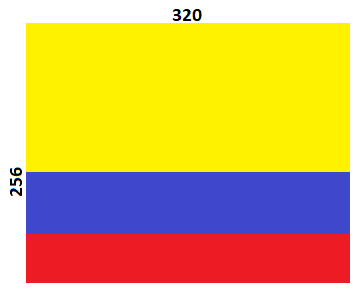
\includegraphics[width=10cm]{ejemplo320x256.png}
    \centering
    \caption{Ejemplo de una imagen 320x256}
    \label{fig:ejemplo1}
    \end{figure}
Luego de dividir de tener los resultados de las divisiones se procederá a recorrer la imagen dando saltos en X de ancho/anchoMatriz y en Y de alto/altomatriz, estos saltos tienen como fin tomar el color del píxel donde estan, dicho color será el que formará parte de la matriz de leds, como se muestra en la figura(\ref{fig:ledrelevante}) con color verde.
    \begin{figure}[h]
    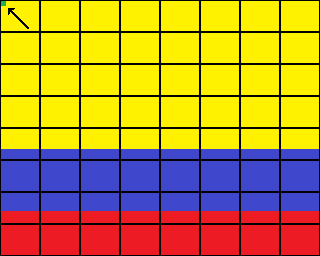
\includegraphics[width=8cm]{ledImportante.png}
    \centering
    \caption{Led relevante.}
    \label{fig:ledrelevante}
    \end{figure}

\subsection{Sobremuestreo}
Para el problema en que la imagen sea más pequeña que la matriz de leds se deberá realizar el proceso de sobremuestreo, para este se ha hecho el siguiente análisis.
Primero se hará un proceso similar al sobremuestreo, pero al contrario del sobremuestreo, aquí no se dividirá por el ancho de la matriz de leds, sino que se tomaran intervalos fijos de dos leds, para después posicionar el color dicho led en la posición siguiente a el.

\end{document}